%%%%%%
%
% $Autor: Wings $
% $Datum: 2020-01-18 11:15:45Z $
% $Pfad: WuSt/Skript/Produktspezifikation/powerpoint/ImageProcessing.tex $
% $Version: 4620 $
%
%%%%%%

%Quelle: https://towardsdatascience.com/deep-learning-framework-power-scores-2018-23607ddf297a
%\url{https://www.kdnuggets.com/2019/05/which-deep-learning-framework-growing-fastest.html}
% \url{https://www.kdnuggets.com/2017/08/pytorch-tensorflow.html}

%todo    \href{https://docs.aws.amazon.com/de_de/machine-learning/latest/dg/step-1-download-edit-and-upload-data.html}{Amazon ML}
%todo https://www.ibm.com/de-de/products/trials


\chapter{Frameworks und Bibliotheken}
\index{Frameworks}
\index{Bibiotheken}


%todo
%todo \section{Kriterien}
%todo https://towardsdatascience.com/deep-learning-framework-power-scores-2018-23607ddf297a


Als Programmiersprache für Data Science stellt Python einen Kompromiss zwischen der Sprache R, die sich schwerpunktmäßig auf Datenanalyse und -visualisierung konzentriert, und Java, die as Rückgrat vieler großangelegter Anwendungen bildet, dar. Diese Flexibilität bedeutet, dass Python als ein einziges Tool fungieren kann, dass Ihren gesamten Workflow zusammenführt.

Python ist häufig die erste Wahl für Entwickler, die bei ihrer Arbeit statistische Techniken oder Datenanalysen anwenden müssen, oder für Datenwissenschaftler, deren Aufgaben in Webanwendungen oder Produktionsumgebungen integriert werden müssen. Python glänzt insbesondere im Bereich des maschinellen Lernens. Die Kombination aus maschinellen Lernbibliotheken und Flexibilität macht Python einzigartig. Python ist bestens geeignet für die Entwicklung von anspruchsvollen Modellen und Vorhersagemodule, die direkt in Produktionssysteme eingebunden werden können.

Eine der größten Stärken von Python ist die umfangreiche Bibliothek. Bibliotheken sind Sätze von Routinen und Funktionen, die in einer bestimmten Sprache geschrieben sind. Ein robuster Satz von Bibliotheken kann die Arbeit von Entwicklern ungemein erleichtern, komplexe Aufgaben auszuführen, ohne viele Codezeilen umschreiben zu müssen. 



\section{Entwicklungsumgebung}


\subsection{Jupyter-Notebook}
\index{Jupyter-Notebook}

Mit der Applikation Jupyter-Notebook kann eine Datei in einem Webbrowser erzeugt werden. Der Vorteil hierbei ist, dass Programme in kleinere Programmabschnitte unterteilt und abschnittsweise ausgeführt werden können. Hierdurch wird das Arbeiten sehr interaktiv. Zudem bietet das Notebook die Möglichkeit Python Programmcodes mit zusätzlichen Textanmerkungen zu
versehen. \cite{Buxmann:2019}




\section{Frameworks}







\subsection{TensorFlow}
\index{TensorFlow}


Das Framework TensorFlow, das von Google unterstützt wird, ist der unangefochtene Platzhirsch. Es hat die meisten GitHub-Aktivitäten, Google-Suchen, Medium-Artikel, Bücher über Amazon und ArXiv-Artikel. Es hat auch die meisten Entwickler, die es benutzen, und ist in den meisten Online-Stellenbeschreibungen aufgeführt. \cite{GoogleTensorFlow:2019}

Für TensorFlow existieren auch Variante, die speziell auf eine Hardware zugeschnitten ist. So werden die Grafikkarten von NVIDIA durch eine Variante mit \ac{cuda} angesprochen und auch Intel hat eine optimierte Variante. Allerdings muss man gegebenenfalls auf die aktuellste Version verzichten.

TensorFlow Lite, die Version für kleine Geräte, bringt die Modellausführung auf eine Vielzahl von Geräten, einschließlich mobiler Geräte und IoT, und bietet eine mehr als 3-fache Steigerung der Inferenzgeschwindigkeit im Vergleich zum ursprünglichen TensorFlow. 

TensorFlow verwendet Datenflussgraphen zur Darstellung der Berechnung, des gemeinsamen Zustands und der Operationen, die diesen Zustand mutieren. Durch die vollständige Darstellung der Abhängigkeiten der einzelnen Berechnungsschritte können Teile der Berechnung zuverlässig parallelisiert werden \cite{Abadi:2016}. 
Ursprünglich sollte TensorFlow für den internen Gebrauch von Google verwendet werden, doch wurde
es im November 2015 unter dem Namen Apache-2.0-Open-Source-Lizenz veröffentlicht.
Seither vereint TensorFlow eine Vielzahl an Werkzeugen, Bibliotheken und Communities.
TensorFlow bietet low-Level Schnittstellen für Programmiersprachen wie Python, Java,
C++ und Go. In den mid-Level und high-Level APIs werden Funktionen zum Erstellen,
Trainieren, Speichern und Laden von Modellen bereitgestellt. \cite{Chollet:2018} %[Men16] 

\begin{figure}[htb]
	\centering
	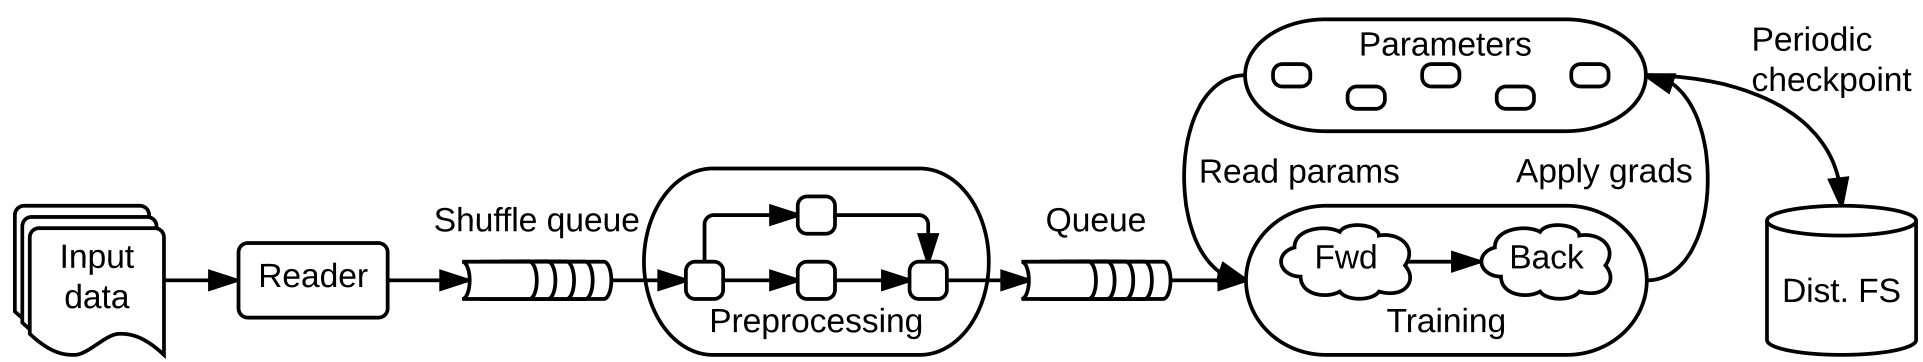
\includegraphics[width=\textwidth]{CUDA/tensorflow-flow-graph.PNG}
	\caption[Tensorflow Datenflussdiagramm]{Tensorflow Datenflussdiagramm \cite{Abadi:2016}}
	\label{fig:tensorflow-flow}
\end{figure}



\subsection{TensorFlow Lite}
\index{TensorFlow Lite}

Tensorflow Lite ist eine, für mobile Geräte und das \ac{iot}, optimierte Umgebung für TensorFlow-Modelle. Im wesentlichen besteht diese aus zwei Komponenten: dem Converter, welcher vortrainierte TensorFlow-Modelle in optimierte TensorFlow Lite-Modelle konvertiert und der Interpreter, welcher die optimierte Ausführung auf den verschiedenen Endgeräten ermöglicht. Das Ziel hierbei ist, die bestehenden Modelle größentechnisch zu reduzieren, sowie die Latenz auf leistungsschwächeren Geräten zu verringern \cite{GoogleTensorFlowLiteGuide:2020}.

\subsection{TensorRT}\label{sec:tensorrt}
\index{TensorRT}

Bei TensorRT handelt es sich um eine auf \ac{cuda} basierte Laufzeitumgebung für neuronale Netze, welche auf die Optimierung der Performance von neuronalen Netzen spezialisiert ist \cite{TensorRT:2015}. Dies wird durch die Verringerung der Berechnungsgenauigkeit von \ac{fp32} auf \ac{fp16} bwz. \ac{int8} erreicht. Da die verbleibende Interferenzgenauigkeit für die meisten Anwendungsfälle ausreichend ist, kann mit diesem Verfahren die Geschwindigkeit deutlich erhöht werden \cite{Gysel:2016}. Bei der Optimierung des Netzes werden die verwendeten Operatoren durch TensorRT Operatoren ausgetauscht, welche nur innerhalb einer TensorRT-Umgebung ausgeführt werden können.


\subsection{Keras}
\index{Keras}

Keras ist eine in Python erstellte High-Level \ac{api} application programming interface (API) für neuronale Netze, die auf TensorFlow, Theano oder CNTK ausgeführt wird. Es ermöglicht das Definieren und Trainieren von unterschiedlichen Deep-Learning-Modellen mit Hilfe  von optimierten Tensor-Bibliotheken, die als Backend-Engine dienen. Unterstützt werden derzeit die Implementierungen TensorFlow-Backend, Theano-Backend und CNTK-Backend. 
Jeglicher in Keras geschriebener Code kann ohne Anpassungen auf den Backends ausgeführt werden. Keras bietet eine Auswahl an vordefinierten Schichten, Optimierungsfunktionen oder weiterer wichtiger Bestandteile von neuronalen Netzen. Die Funktionen können zudem mit eigenen Modulen erweitert werden. Die wichtigsten zwei Modelltypen, die Keras bereitstellt sind sequential und functional api. Mit sequential lassen sich gradlinige Modelle erstellen deren Schichten hintereinander gereiht sind. Für komplexere Netzstrukturen mit Rückführungen gibt es die functional api. \cite{Chollet:2018,Keras:2020}

\subsection{PyTorch}
\index{PyTorch}

PyTorch, das von Facebook unterstützt wird,  ist das drittbeliebteste Framework. Es ist jünger als TensorFlow und hat rasch an Popularität gewonnen. Es erlaubt eine Anpassung, die TensorFlow nicht erlaubt. \cite{PyTorch:2020}


\subsection{Caffe}
\index{Caffee}

Caffe gibt es seit fast fünf Jahren. Es wird von Arbeitgebern relativ stark nachgefragt und häufig in wissenschaftlichen Artikeln erwähnt, hat aber in jüngster Zeit kaum über seine Verwendung berichtet.
\cite{Caffe:2020}

\subsection{Caffe2}
\index{Caffee2}

Caffe2 ist ein weiteres Open-Source-Produkt von Facebook. Es baut auf Caffe auf und befindet sich nun im PyTorch GitHub-Repository. \cite{Caffe2:2020}

\subsection{Theano}
\index{Theano}

Theano wurde 2007 an der Universität von Montreal entwickelt und ist das älteste bedeutende Python-Framework. Es hat viel von seiner Popularität eingebüßt, und sein Leiter erklärte, dass Hauptversionen nicht mehr auf dem Fahrplan stünden. Es werden jedoch weiterhin Aktualisierungen vorgenommen. \cite{Theano:2016}

Theano verwendet eine NumPy-ähnliche Syntax, um mathematische Ausdrücke zu optimieren und auszuwerten. Was Theano unterscheidet, ist, dass es die \ac{gpu} der Grafikkarte des Computers nutzt.
 Die Geschwindigkeit macht Theano somit interessant.

\subsection{Apache MXNet}
\index{MXNet}

MXNET wird von Apache unterstützt und von Amazon genutzt. \cite{MXNet:2020}
\index{Amazon}

\subsection{CNTK}
\index{CNTK}

CNTK ist das Microsoft Cognitive Toolkit\index{Microsoft Cognitive Toolkit}. Es erinnert mich an viele andere Microsoft-Produkte in dem Sinne, dass es versucht, mit Google- und Facebook-Angeboten zu konkurrieren und keine nennenswerte Akzeptanz findet. \cite{CNTK:2020}

\subsection{Deeplearning4J}

\index{Deeplearning4J}

Deeplearning4J, auch DL4J genannt, wird mit der Sprache Java verwendet. Es ist das einzige halbpopuläre Framework, das nicht in Python verfügbar ist. Sie können jedoch Modelle, die mit Keras geschrieben wurden, in DL4J importieren. Das Framework besitzt eine Anbindung zu Apache Spark und Hadoop. \cite{Deeplearning4J:2020}


\subsection{Chainer}
\index{Chainer}

Chainer ist ein Framework, das von der japanischen Firma Preferred Networks entwickelt wurde. Es hat eine kleine Fangemeinde. \cite{Chainer:2020}

\subsection{FastAI}
\index{FastAI}

FastAI baut auf PyTorch. Seine API wurde von Keras inspiriert und erfordert noch weniger Code für starke Ergebnisse.  Jeremy Howard, die treibende Kraft hinter Fast.AI, war ein Top-Kaggler und Präsident von Kaggle. \cite{FastAI:2020}

Fast.AI ist bisher weder für Karrieren gefragt, noch wird es breit eingesetzt. Es hat jedoch eine große eingebaute Pipeline von Benutzern durch seine beliebten kostenlosen Online-Kurse. Außerdem ist es sowohl leistungsstark als auch einfach zu benutzen. Seine Akzeptanz könnte erheblich zunehmen.

\section{Allgemeine Bibliotheken}

Dies sind die grundlegenden Bibliotheken, die Python von einer universellen Programmiersprache in ein leistungsfähiges und robustes Werkzeug für die Datenanalyse und -visualisierung verwandeln. Sie werden manchmal als SciPy-Stapel bezeichnet und bilden die Grundlage für die Spezialwerkzeuge.


\subsection{NumPy}
\index{NumPy}


NumPy ist die grundlegende Bibliothek für wissenschaftliches Rechnen in Python, und viele der Bibliotheken in dieser Liste verwenden NumPy-Arrays als grundlegende Ein- und Ausgänge. Kurz gesagt, NumPy führt Objekte für mehrdimensionale Arrays und Matrizen ein, sowie Routinen, die es Entwicklern erlauben, erweiterte mathematische und statistische Funktionen auf diesen Arrays mit so wenig Code wie möglich auszuführen. \cite{Python:2020c}


\subsection{SciPy}
\index{SciPy}

SciPy baut auf NumPy auf, indem es eine Sammlung von Algorithmen und High-Level-Befehlen zur Manipulation und Visualisierung von Daten hinzufügt. Das Paket enthält außerdem Funktionen zur numerischen Berechnung von Integralen, zur Lösung von Differentialgleichungen, Optimierung und mehr.

\subsection{Pandas}
\index{Pandas}

Pandas fügt Datenstrukturen und Werkzeuge hinzu, die für die praktische Datenanalyse in Finanz-, Statistik-, Sozial- und Ingenieurwissenschaften konzipiert sind. Pandas eignet sich gut für unvollständige, unordentliche und unmarkierte Daten (d. h. Für die Art von Daten, mit denen Sie wahrscheinlich in der realen Welt konfrontiert werden) und bietet Werkzeuge zum Formen, Zusammenführen, Umformen und Aufteilen von Datensätzen.

\subsection{IPython}
\index{IPython}

IPython erweitert die Funktionalität von Pythons interaktivem Interpreter um eine aufgemotzte interaktive Shell, die Introspektion, Rich Media, Shell-Syntax, Tab-Vervollständigung und Befehlsarchiv-Abruf ergänzt. Es fungiert auch als ein integrierter Interpreter für Ihre Programme, der insbesondere für das Debuggen nützlich sein kann. Wenn man jemals Mathematica oder MATLAB verwendet haben, so wird man sich mit IPython wohlfühlen.

\subsection{Matplotlib}
\index{Matplotlib}

Matplotlib ist die Standard-Python-Bibliothek zum Erstellen von 2D-Diagrammen und Diagrammen. Die API ist ziemlich low-level, d.h. es erfordert mehrere Befehle, um gut aussehende Graphen und Zahlen zu erzeugen im Vergleich zu einigen   fortgeschritteneren Bibliotheken. Der Vorteil ist jedoch eine größere Flexibilität. Mit genügend Befehlen kann man mit matplotlib fast jede beliebige Grafik erstellen.




\subsection{scikit-learn}
\index{scikit-learn}

scikit-learn baut auf NumPy und SciPy auf, indem es eine Reihe von Algorithmen für allgemeine maschinelle Lern- und Data Mining-Aufgaben hinzufügt, einschließlich Clustering, Regression und Klassifizierung. Als Bibliothek hat scikit-learn viel zu bieten. Seine Werkzeuge sind gut dokumentiert und unter den mitwirkenden Entwicklern sind viele Maschine Learning Experten. Darüber hinaus ist es eine sehr hilfreiche Bibliothek für Entwickler, die nicht zwischen verschiedenen Versionen desselben Algorithmus wählen möchten. Durch seine Mächtigkeit und Benutzerfreundlichkeit ist die Library sehr beliebt.



\subsection{Scrapy}
\index{Scrapy}

Scrapy ist eine Bibliothek zum Erstellen von Spiderbots, um das Web systematisch zu crawlen und strukturierte Daten wie Preise, Kontaktinformationen und URLs zu extrahieren. Ursprünglich für Web Scraping entwickelt, kann Scrapy auch Daten aus APIs extrahieren.

\subsection{NLTK}
\index{NLTK}

NLTK steht für Natural Language Toolkit und ermöglicht den effektiven Einstieg ins Natural Language Processing (NLP) bzw. Text Mining mit Python.
Die grundlegenden Funktionen von NLTK ermöglichen es Ihnen, Text zu markieren, benannte Entitäten zu identifizieren und Parser-Bäume anzuzeigen, die wie Satzdiagramme Teile von Sprache und Abhängigkeiten aufdecken. Somit erhält man die Möglichkeit, kompliziertere Dinge wie Sentiment-Analysen durchzuführen oder automatische Textzusammenfassungen zu generieren.

 
\subsection{Pattern}
\index{Pattern}

Pattern kombiniert die Funktionalität von Scrapy und NLTK in einer umfangreichen Bibliothek, die als Out-of-the-Box-Lösung für Web-Mining, NLP, maschinelles Lernen und Netzwerkanalyse dienen soll. Zu seinen Tools gehören ein Web-Crawler; APIs für Google, Twitter und Wikipedia; und Textanalysealgorithmen wie Parsebäume und Sentiment Analysen, die mit nur wenigen Codezeilen ausgeführt werden können.

\subsection{Seaborn}
\index{Seaborn}

Seaborn ist eine beliebte Visualisierungsbibliothek, die auf der Grundlage von matplotlib aufbaut. Mit Seaborn sind grafisch sehr hochwertige Plots wie Heat Maps, Zeitreihen und Violin-Plots generierbar.

\subsection{Bokeh}
\index{Bokeh}

Bokeh ermöglicht die Erstellung interaktive, zoombare Diagramme in modernen Webbrowsern mithilfe von JavaScript-Widgets. Ein weiteres nettes Feature von Bokeh ist, dass es mit drei Ebenen der Benutzeroberfläche, von High-Level-Abstraktionen, mit denen Sie schnell komplexe Plots erstellen können, bis hin zu einer Low-Level-Ansicht, die maximale Flexibilität für App-Entwickler bietet.

\subsection{Basemap}
\index{Basemap}

Basemap unterstützt das Hinzufügen einfacher Karten zu matplotlib, indem die Koordinaten von matplotlib übernommen und auf mehr als 25 verschiedene Projektionen angewendet werden. Die Bibliothek Folium baut auf Basemap auf und ermöglicht die Erstellung von interaktiven Webkarten, ähnlich den JavaScript-Widgets von Bokeh.

\subsection{NetworkX}
\index{NetworkX}

Mit dieser Bibliothek kann man Graphen und Netzwerke erstellen und analysieren. Es wurde entwickelt, um sowohl mit standardmäßigen als auch mit nicht standardmäßigen Datenformaten zu arbeiten, was es besonders effizient und skalierbar macht. Mit diesem Features ist NetworkX besonders gut geeignet zur Analyse komplexer sozialer Netzwerke.

\subsection{LightGBM}
\index{LightGBM}

Gradient Boosting gehört zu den besten und beliebtesten Bibliotheken für Machine Learning und hilft Entwicklern dabei neue Algorithmen zu erstellen, indem sie neu definierte Elementarmodelle und insbesondere decision treesverwenden.

Dementsprechend gibt es spezielle Bibliotheken, die für eine schnelle und effiziente Implementierung dieser Methode ausgelegt sind. Diese sind LightGBM, XGBoost und CatBoost. All diese Bibliotheken sind Konkurrenten, helfen aber ein gemeinsames Problem zu lösen und können auf fast ähnliche Weise verwendet werden.

\subsection{Eli5}
\index{Eli5}

Meistens sind die Ergebnisse von Modellvorhersagen beim Machine Learning nicht wirklich genau. Die in Python integrierte Bibliothek Eli5 hilft bei der Bewältigung genau dieser Herausforderung. Es ist eine Kombination aus Visualisierung und Debugging aller Modelle für maschinelles Lernen und Tracking aller Arbeitsschritte des Algorithmus.

\subsection{Mlpy – Machine Learning}
\index{Mlpy}

Alternativ zu scikit-learn, bietet auch Mlpy eine mächtige Bibliothek an Funktionen für Machine Learning. Mlpy setzt ebenfalls auf NumPy und SciPy, auf, erweitert den Funktionsumfang jedoch um Methoden des überwachten und unüberwachten maschinellen Lernens.

\subsection{Statsmodels – Statistische Datenanalyse}
\index{Statsmodels}

Statsmodels ist ein Python-Modul, mit dem Benutzer Daten untersuchen, statistische Modelle schätzen und statistische Tests durchführen können. Eine umfangreiche Liste beschreibender Statistiken, statistischer Tests, Plotting-Funktionen und Ergebnisstatistiken steht für verschiedene Datentypen und jeden Schätzer zur Verfügung.
Mit dem Modul wird Predictive Analytics möglich. Statsmodels wird häufig mit NumPy, matplotlib und Pandas kombiniert.


\section{Spezielle Bibliotheken}


\subsection{OpenCV}
\index{OpenCV}


OpenCV, abgeleitet für Open Computer Vision, ist eine freie Programmbibliothek mit Algorithmen für die Bildverarbeitung und Computer Vision. Die Entwicklung der Bibliothek wurde von Intel initiiert und wurde bis 2013 von Willow Garage gepflegt. Nach deren Auflösung wurde sie von Itseez fortgeführt, welches mittlerweile von Intel übernommen wurde. \cite{OpenCV:2020b}


\subsection{OpenVINO}
\index{OpenVINO}

Das OpenVINO-Toolkit hilft bei der beschleunigten Entwicklung von leistungsfähiger Computervision und dem Deep Learning in Visionsanwendungen. Es ermöglicht Deep Learning über Hardwarebeschleuniger sowie eine einfache, heterogene Ausführung auf Intel-Plattformen, darunter ac{cpu}, \ac{gpu}, \ac{fpga} und \ac{vpu}. Zu den Hauptkomponenten gehören optimierte Funktionen für OpenCV.
\cite{IntelRequirements:2019,OpenVino:2020}

\subsection{\ac{cuda}}



Die Abkürzung \ac{cuda} steht für Compute Unified Device Architecture. Es handelt sich um eine Schnittstellentechnologie und Computing-Plattform, mit der sich Grafikprozessoren ansprechen und auch für nicht grafikspezifische Berechnungen nutzen lassen. \ac{cuda} wurde von NVIDIA entwickelt und beschleunigt Programme, indem neben der \ac{cpu} bestimmte Programmteile von einer oder mehreren \ac{gpu}s parallelisiert bearbeitet werden. \cite{Tan:2019,CUDA:2020,CUDATK:2020} 

\subsection{OpenNN}
\index{OpenNN}

OpenNN ist eine in C++ geschriebene Software-Bibliothek für fortgeschrittene Analysen. Sie implementiert neuronale Netze.
Diese Bibliothek zeichnet sich durch ihre Ausführungsgeschwindigkeit und Speicherzuweisung aus. Sie wird ständig optimiert und parallelisiert, um ihre Effizienz zu maximieren. \cite{OpenNN:2020}
	




\section{Besondere Bibliotheken}

Bei der Programmierung des neuronalen Netzes wird auf einige, vordefinierte Bibliotheken 
zugegriffen. Im Nachfolgenden werden die einige interessante Bibliotheken vorgestellt.

\subsection{glob}
\index{glob}

Das glob-Modul findet alle Pfadnamen in einem bestimmten Verzeichnis, die mit einem
angegeben Muster übereinstimmen und gibt diese in willkürlicher Weise wieder. \cite{Python:2020}

\subsection{os}
\index{os}

Mit dem os-Modul werden allgemeine Betriebssystemfunktionalitäten zur Verfügung gestellt. 
Die Funktionen dieser Bibliothek erlauben es Programme plattformunabhängig zu
gestalten. Die Abkürzung os steht für Operating System. Es ermöglicht den Zugriff und
das Verweisen auf bestimmte Pfade und die dort hinterlegten Dateien. \cite{Balakreshnan:2019}

\subsection{PIL}
\index{PIL}

Die Abkürzung PIL steht für Python Image Libary und stellt viele Funktionen für die
Bildverarbeitung zur Verfügung. Es wird ein schneller Datenzugriff auf die grundlegenden
Bildformate gewährleistet. Neben Bildarchivierungs- und Stapelfunktionsanwendungen
können auch Dateiformate konvertiert, Miniaturansichten erstellt, Bilder gedruckt und
viele weitere Funktionen durchgeführt werden. \subsection{LCC15}

\subsection{math}
\index{math}

Wie sich aus dem Namen leicht entnehmen lässt, ermöglicht diese Bibliothek Zugriff auf
alle in der C-Norm definierten mathematischen Funktionen. Hierzu zählen unter anderem
die trigonometrischen Funktionen, Potenz- und Logarithmusfunktionen und Winkelfunk-
tionen. Komplexe Zahlen sind in dieser Bibliothek nicht enthalten. \cite{Python:2020c}


\subsection{cv2}
\index{cv2}

Mit dem cv2-Modul können Eingangsbilder in dreidimensionale Arrays umgeschrieben
werden. OpenCV beinhaltet Algorithmen für die Bildverarbeitung und des maschinellen
Sehens. Die Algorithmen bestehen aus neusten Forschungsergebnissen und werden kontinuierlich 
weiterentwickelt. Die Module aus der Bildbearbeitung umfasst beispielsweise die
Gesichtserkennung, sowie viele schnelle Filter und Funktionen zur Kamerakalibrierung.
Die Module für das maschinelle Sehen beinhaltet Boosting (automatische Klassifizierung),
Lernen eines Entscheidungsbaum und künstliche neuronale Netze. \cite{OpenCV:2020}

\subsection{random}
\index{random}

Das Random-Modul implementiert Pseudozufallszahlengeneratoren für verschiedene Ver-
teilungen. So können zum Beispiel Zufallszahlen erzeugt werden oder eine Durchmischung
von Elementen erzeugt werden. \cite{Python:2020e}

\subsection{pickle}
\index{pickle}

Das pickle-Modul implementiert binäre Protokolle zum Serialisieren und Deserialisieren 
einer Python-Objektstruktur. Objekthierachien können in einem binären Strom konvertiert
(pickle) und anschließend von einer binären Architektur zurück in die objekthierachischen
Struktur gebracht werden (unpickle). \cite{Python:2020d}

\subsection{PyPI}
\index{PyPI}

Die Organisation Python Software Foundation\index{Python Software Foundation} organisiert und verwaltet verschiedene Pakete für die Python-Programmierung. \cite{PyPI:2021} Hier kann man für die verschiedensten Aufgaben fündig werden. Ein Beispiel ist die offizielle \ac{api} für den Zugriff auf den Datensatz \ac{coco}. \cite{PyPI:2021b}



%todo	
%\begin{enumerate}
%	\item ONNX
%	\item Torch
%	\item Accord.NET
%
%	\item Apache Spark
%	\item Apache Mathout
%	\item Apache SINGA
%    \item Apache SystemML \cite{Pansare:2018}
%	
%	\item Gensim
%	\item mlpack
%	\item Mycroft
%	\item DyNet
%	\item Shogun
%\end{enumerate}
